\chapter{Design Methodology}

\begin{comment}
\indent\indent From Chapter 2 onwards, every chapter should start with an introduction paragraph. This paragraph should brief about the flow of the chapter. This introduction can be limited within 4 to 5 sentences. The chapter heading should be appropriately modified (a sample heading is shown for this chapter).But don't start the introduction paragraph in the chapters 2 to end with "This chapter deals with....". Instead you should bring in the highlights of the chapter in the introduction paragraph. 
\end{comment}

Designing efficient ML hardware requires a structured approach to both architectural modeling and accelerator development. This chapter outlines the methodology adopted for evaluating custom FPGA architectures using the VTR toolchain, with a focus on carry chain-based logic for arithmetic-heavy ML benchmarks. In parallel, it details the step-by-step design of the Manojavam PCA accelerator, including its systolic matrix engine, cache hierarchy, and controller structure. Key design decisions, supporting models, experimental workflows, and analytical formulations are also discussed, setting the foundation for implementation and result analysis in the subsequent chapters.

\section{Specifications of FPGA Architectural Exploration}
The motivation behind this architectural exploration stems from the need to understand how the internal composition of FPGA logic blocks — particularly the nature of carry propagation and the use (or absence) of hardened arithmetic units — influences the efficiency of mapping arithmetic-heavy workloads. In the context of machine learning (ML) applications, such as matrix multiplications, digital filters, and accumulation pipelines, the performance of the underlying hardware is highly sensitive to how well the architecture supports fast and compact arithmetic operations. While modern commercial FPGAs like Intel Stratix-10 or Xilinx Versal feature hardened DSP blocks to optimize multiply-accumulate operations, many research-grade or open-source FPGA fabrics, as well as ASIC-grade RTL flows, rely instead on carry chains composed of basic logic elements. Studying the tradeoffs between heterogeneous architectures (with DSP hard blocks) and homogeneous logic-only designs (with serial or parallel carry chains) offers insights into how arithmetic-dense applications behave across a broader architectural spectrum.

To facilitate this analysis, three target architectures were employed in the study, each described in the VTR architectural XML format. The first is a Stratix-10-like architecture, modeling hardened multipliers and adder trees to resemble a modern high-performance heterogeneous FPGA. The second is a homogeneous architecture featuring a 4-bit single carry chain, where carry propagation is strictly serial across four 1-bit full adders, emulating delay-intensive arithmetic behavior. The third is a 4-bit double carry chain architecture that introduces parallel carry propagation paths, allowing partial carries to resolve concurrently, thus improving throughput for wider additions. These three configurations allow us to explore the performance spectrum from hardened, low-latency arithmetic to logic-only, delay-sensitive arithmetic styles.

All three architectures were evaluated under a fixed routing and interconnect model — specifically, a standard island-style routing architecture as defined in VTR. Each architecture maintains the same routing switch box style, wire segmentation, and global resource availability. The only changes lie in the logic block definitions — namely, the composition of BLEs (basic logic elements), the presence or absence of carry chains, and how multipliers are realized (hardened vs. synthesized). This isolation of variables ensures that performance differences are directly attributable to logic architecture rather than routing artifacts or placement constraints.

To assess the practical implications of these architectural differences, a fixed set of HDL benchmarks were synthesized and mapped onto each architecture. These benchmarks consist of:
\begin{enumerate}
	\item \textbf{Adder Trees:} 2-level and 3-level summation trees for fixed-point operands, stressing chained addition performance.
	\item \textbf{FIR Filters:} Pipelined and unpipelined FIR structures with and without hard multipliers. For carry-based architectures, multipliers were implemented using Wallace-tree style adder networks, exercising the carry chain fabric intensively.
\end{enumerate}

Performance was quantified using three key metrics:
\begin{enumerate}
	\item \textbf{Operational Frequency (f)} — defined as the reciprocal of the longest delay path:
	\item \textbf{Critical Path Delay (D)} — the maximum timing delay (in nanoseconds) from any input to output in the post-place-and-route design.
	\item \textbf{Area (MWTA)}  — a weighted logic utilization model inspired by VTR
\end{enumerate}

This setup provides a controlled environment to understand how different logic architectures influence the performance of ML-relevant workloads, enabling data-driven decisions for future FPGA or domain-specific accelerator designs.

\section{FPGA Architectural Modeling in VTR}
To perform a rigorous architectural exploration, three FPGA fabric configurations were modeled using the Verilog-to-Routing (VTR) toolchain: (1) Intel Stratix-10-like heterogeneous FPGA with hardened DSP blocks, (2) a homogeneous FPGA with a 4-bit carry chain within each logic block (single chain), and (3) a variant with two parallel 4-bit carry chains (double chain). These configurations were described using VTR’s XML-based architecture specification language, with a focus on modeling complex logic blocks (CLBs), interconnects, and hard blocks like multipliers and memories.

\subsection{CLB Architecture and Carry Chain Design}
At the heart of each fabric lies its CLB (Configurable Logic Block) design. In the Stratix-10 model, the CLB closely mimics Intel’s Adaptive Logic Module (ALM), which includes 6-input fracturable LUTs and dedicated hardened carry logic. The carry chains here are tightly coupled with the LUT outputs, and propagate between logic elements using explicitly defined \textbf{direct} connections — one for incoming carry from the previous LAB and another for chaining between elements within a CLB. The structure supports efficient arithmetic mapping and pipelining in DSP-like workloads

The 4-bit single chain architecture departs from this by implementing a simplified carry chain that connects five logic elements linearly within a single chain per CLB. The XML model defines a chain pattern from \textbf{fle1[0].cout} to \textbf{fle1[1].cin}, and so on, terminating at \textbf{fle1[4]}. The carry-in for this chain originates from an external \textbf{cin} pin on the CLB, and the carry-out from the last element is routed to \textbf{cout}. This mimics the operation of older generation FPGAs or minimalist logic fabrics where a single chain is adequate for low-to-medium complexity arithmetic.

The double chain architecture enhances this further by including two parallel 4-bit chains, allowing for simultaneous arithmetic operations across two independent data paths. This is evident from how two sets of fle instances are used \textbf{(fle[0:4] and fle[5:9])}, each having its own \textbf{cin} and \textbf{cout} wiring paths. The interconnect model explicitly defines chaining within each set as well as the routing from the LAB to the CLB inputs and outputs, capturing parallelism in low-precision arithmetic mapping.

\subsection{Routing and Interconnects}
All three architectures share a uniform island-style routing structure characterized by segmented wires, programmable switch boxes, and connection blocks. The routing tracks are uniformly distributed across the horizontal (x) and vertical (y) directions with a peak utilization factor of 1.0. Wilton-style switch blocks were used \textbf{(fs=3)} to enable flexible connectivity and short detours around congested regions, and \textbf{ipin-cblock} switches were employed for linking routing wires to logic block inputs. This standardization ensures that any differences in performance metrics can be attributed primarily to the internal CLB and carry chain design rather than the routing infrastructure.

\subsection{Hardblocks and Memory Modeling}
Across all architectures, the multiplier logic is defined using a \textbf{pb-type} block for a 27×27-bit fracturable multiplier. Internally, this multiplier can operate in multiple modes: two 18×19-bit multipliers or one 27×27-bit unit, reflecting the flexibility of real-world DSP blocks. These modes enable trade-offs between precision and resource utilization. The internal delay characteristics are also modeled, with a delay of approximately 1.825 ns for each 18×19 multiplier, aligning with data from Intel Arria-10 chips fabricated in 22nm technology nodes.

Memory blocks, though not heavily emphasized in this study, are modeled as simple RAM blocks with fixed delays. These provide compatibility with workloads such as FIR filters and adder trees that may require coefficient or state storage.

In essence, this section formalizes the modeling of three FPGA architectural variants in VTR, emphasizing differences in CLB composition and carry chain capabilities. While the routing, memory, and multiplier subsystems were kept largely consistent, the varying styles of arithmetic support within the logic blocks allowed us to examine their influence on performance and area when mapped with arithmetic-heavy benchmarks. These architecture files served as the foundation for place-and-route trials, allowing us to extract meaningful comparisons across design metrics such as critical path delay, logic utilization, and peak operating frequency.

\section{Methodology for FPGA Architectural Exploration using VTR}
To evaluate how different FPGA architectures handle machine learning-oriented workloads, the Verilog-to-Routing (VTR) toolchain was employed as the core design exploration framework. This methodology aimed to systematically analyze architectural features—particularly carry chains and DSP-based blocks—and their effect on logic utilization, timing, and packing behavior across a series of ML-inspired benchmarks. The complete flow begins with Verilog-based HDL descriptions of the benchmark circuits, followed by synthesis, logic optimization, physical design using VPR, and ends with extraction and comparative analysis of key performance metrics.

The input to the flow consists of Verilog modules representing arithmetic-dominated circuits such as adder trees and FIR filters. These were either directly synthesized using ODIN-II, which is integrated into the VTR toolchain, or preprocessed using Yosys when finer control over synthesis was required—particularly in cases where multiplication operators were explicitly replaced with adder networks to force logic mapping onto carry chains. This preprocessing helped standardize the structure of the circuits, ensuring that architecture-dependent variations observed in later stages were genuine and not synthesis artifacts.

Post synthesis, the resulting intermediate logic network is passed through ABC, a logic optimization and technology mapping tool that is tightly integrated with VTR. ABC performs a series of transformations to simplify and balance the logic, minimize delay, and prepare the design for physical mapping. The output of this step is a BLIF (Berkeley Logic Interchange Format) file, which represents the optimized netlist and becomes the primary input to the placement and routing stages of the flow.

The next phase of the methodology involves running the BLIF file through the Versatile Place and Route (VPR) engine. VPR operates on a user-defined FPGA architecture specified via XML, which details the structure and interconnect of the logic blocks, switch boxes, routing channels, carry chains, and DSP blocks. In this project, three architecture files were used to model: (1) a baseline Intel Stratix-10–style architecture with hardened DSP blocks, (2) a 4-bit single carry chain architecture where each CLB is equipped with a single serial carry propagation path, and (3) a 4-bit double carry chain architecture that provides enhanced arithmetic throughput through dual carry paths.

The VPR engine performs packing, placement, and routing tailored to the architecture file. The packing stage clusters logic elements into configurable logic blocks (CLBs). For carry chain-based architectures, packing favors tight clustering of adders to exploit localized carry propagation paths, while in DSP-based designs, packing tends to consolidate multiplier-heavy logic into fixed-function DSP blocks. This difference leads to significant architectural trade-offs: carry chain-based designs often offer higher utilization efficiency and better support for low-precision arithmetic, whereas DSP-based architectures perform better for large-width multipliers but may suffer from resource underutilization. After packing, VPR places the clusters on the grid and performs routing to connect them, finally conducting timing analysis to evaluate path delays, clock frequency potential, and signal integrity.

At the conclusion of each run, VPR produces detailed reports that include critical path delay, logic block usage, routing channel widths, switch utilization, and cluster packing efficiency. These metrics serve as the basis for evaluating architectural performance. For example, in adder-dense benchmarks, the carry chain architectures often showed improvements in delay and area metrics due to efficient local routing and minimal use of global interconnects. In contrast, the Stratix-10–style DSP architecture displayed strengths in FIR filters with wide datapaths, though at the cost of higher power and underutilized multiplier blocks for narrower bit-widths.

Given the extensive number of architecture-benchmark combinations, the entire VTR flow was automated using shell scripts, allowing batch execution of synthesis, placement, routing, and report extraction across all benchmark-architecture pairs. This not only reduced manual intervention but also ensured consistency across evaluations, enabling a scalable and repeatable testing framework. In addition to this, a separate Python-based preprocessing pipeline was developed to transform Verilog benchmark designs. Specifically, FIR filter designs that originally used the multiplication \textbf{(*)} operator were programmatically converted into structurally described Wallace tree multipliers, facilitating accurate mapping to carry chain logic and enabling architecture-aware synthesis. This Python module acted as a custom Verilog code generator, automatically restructuring arithmetic-heavy blocks to reflect fine-grained logic suitable for low-bit-width architectures. These preprocessed designs, when passed through the VTR flow, provided insights into how architectural choices affect resource utilization and timing when optimized arithmetic representations are employed.

\section{FPGA Analysis Metrics Equations}
In order to quantitatively evaluate and compare the performance of different FPGA architectures for ML-relevant workloads, three primary metrics were employed in this study: Operational Frequency, Critical Path Delay, and Area in MWTA (Minimum Width Transistor Area). These metrics are derived from the post-routing reports generated by the VTR toolchain and offer insights into the timing performance and spatial efficiency of each architecture.

\subsection{Operational Frequency}
Operational frequency indicates the maximum clock rate at which the synthesized design can be reliably executed on the given FPGA architecture. It is the inverse of the critical path delay and is computed as:
\begin{equation}
	f_{op} = \frac{1}{T_{cp}}
	\label{eq:operational_Frequency_vtr}
\end{equation}

Where $T_{cp}$ is the critical path delay (in seconds), reported by VPR.

To express $f_{op}$ in MHz, the equation becomes:
\begin{equation}
	f_{op}(MHz) = \frac{10^{3}}{T_{cp}(ns)}
	\label{eq:operational_Frequency_vtr_mhz}
\end{equation}

Where the symbols retain their usual meaning.

\subsection{Critical Path Delay}
The critical path delay refers to the longest path delay through the combinational logic of the design, which determines the minimum possible clock period. This metric reflects the delay bottleneck of the circuit and is a direct output of the VPR timing analysis engine.

\begin{equation}
	T_{cp} = max(\sum_{i}d_{i})
\end{equation}

Where $d_{i}$ is the delay of each logic element and interconnect on a specific path. 

\subsection{Area in MWTA Units}
Area is measured in terms of Minimum Width Transistor Area (MWTA), a normalized metric used by VTR to estimate the silicon area occupied by the design on a theoretical FPGA fabric. MWTA is a technology-independent metric that allows fair comparison across architectures.

The Area in MWTA units is described in the equation below:
\begin{equation}
	A_{MWTA} = \sum_{i}(Area_{block_i}) + \sum_{j}(Area_{routing_j})
\end{equation}

Where $Area_{block_i}$ includes the area of logic blocks, flip-flops, and DSPs, and $Area_{routing_j}$ includes switch boxes, connection boxes, and wire segments.

This metric provides a coarse estimation of the physical footprint and is particularly useful in evaluating the area efficiency of logic structures such as carry chains versus DSP blocks.

Together, these metrics provide a comprehensive basis for analyzing architectural performance. While operational frequency and critical path delay capture timing behavior, the MWTA area metric enables hardware designers to assess the compactness and logic density achieved under each architecture configuration.

\section{Architecture of the Manojavam Accelerator}
The Manojavam PCA accelerator is a fully RTL-based hardware architecture designed to compute Principal Component Analysis in a power-efficient and scalable manner. PCA is a core operation in machine learning pipelines and involves two principal computational steps: covariance matrix computation and eigendecomposition via the Jacobi method. Manojavam is organized into three tightly coupled stages: the Covariance Matrix Computation Unit, the Jacobian Unit, and the Rotation Unit. Together, these components operate on streamed matrix tiles, allowing the accelerator to process large datasets efficiently. A defining characteristic of Manojavam is the reuse of datapaths between the covariance and rotation stages, enabling the architecture to optimize for both area and performance without duplicating compute logic. The complete design is implemented in Verilog HDL, simulated in Vivado, and validated through both FPGA and ASIC (OpenLane) flows. The high level architecture of Manojavam is as shown in Fig.\ref{fig:manojavam high level architecture}.

\begin{figure}
	\centerline{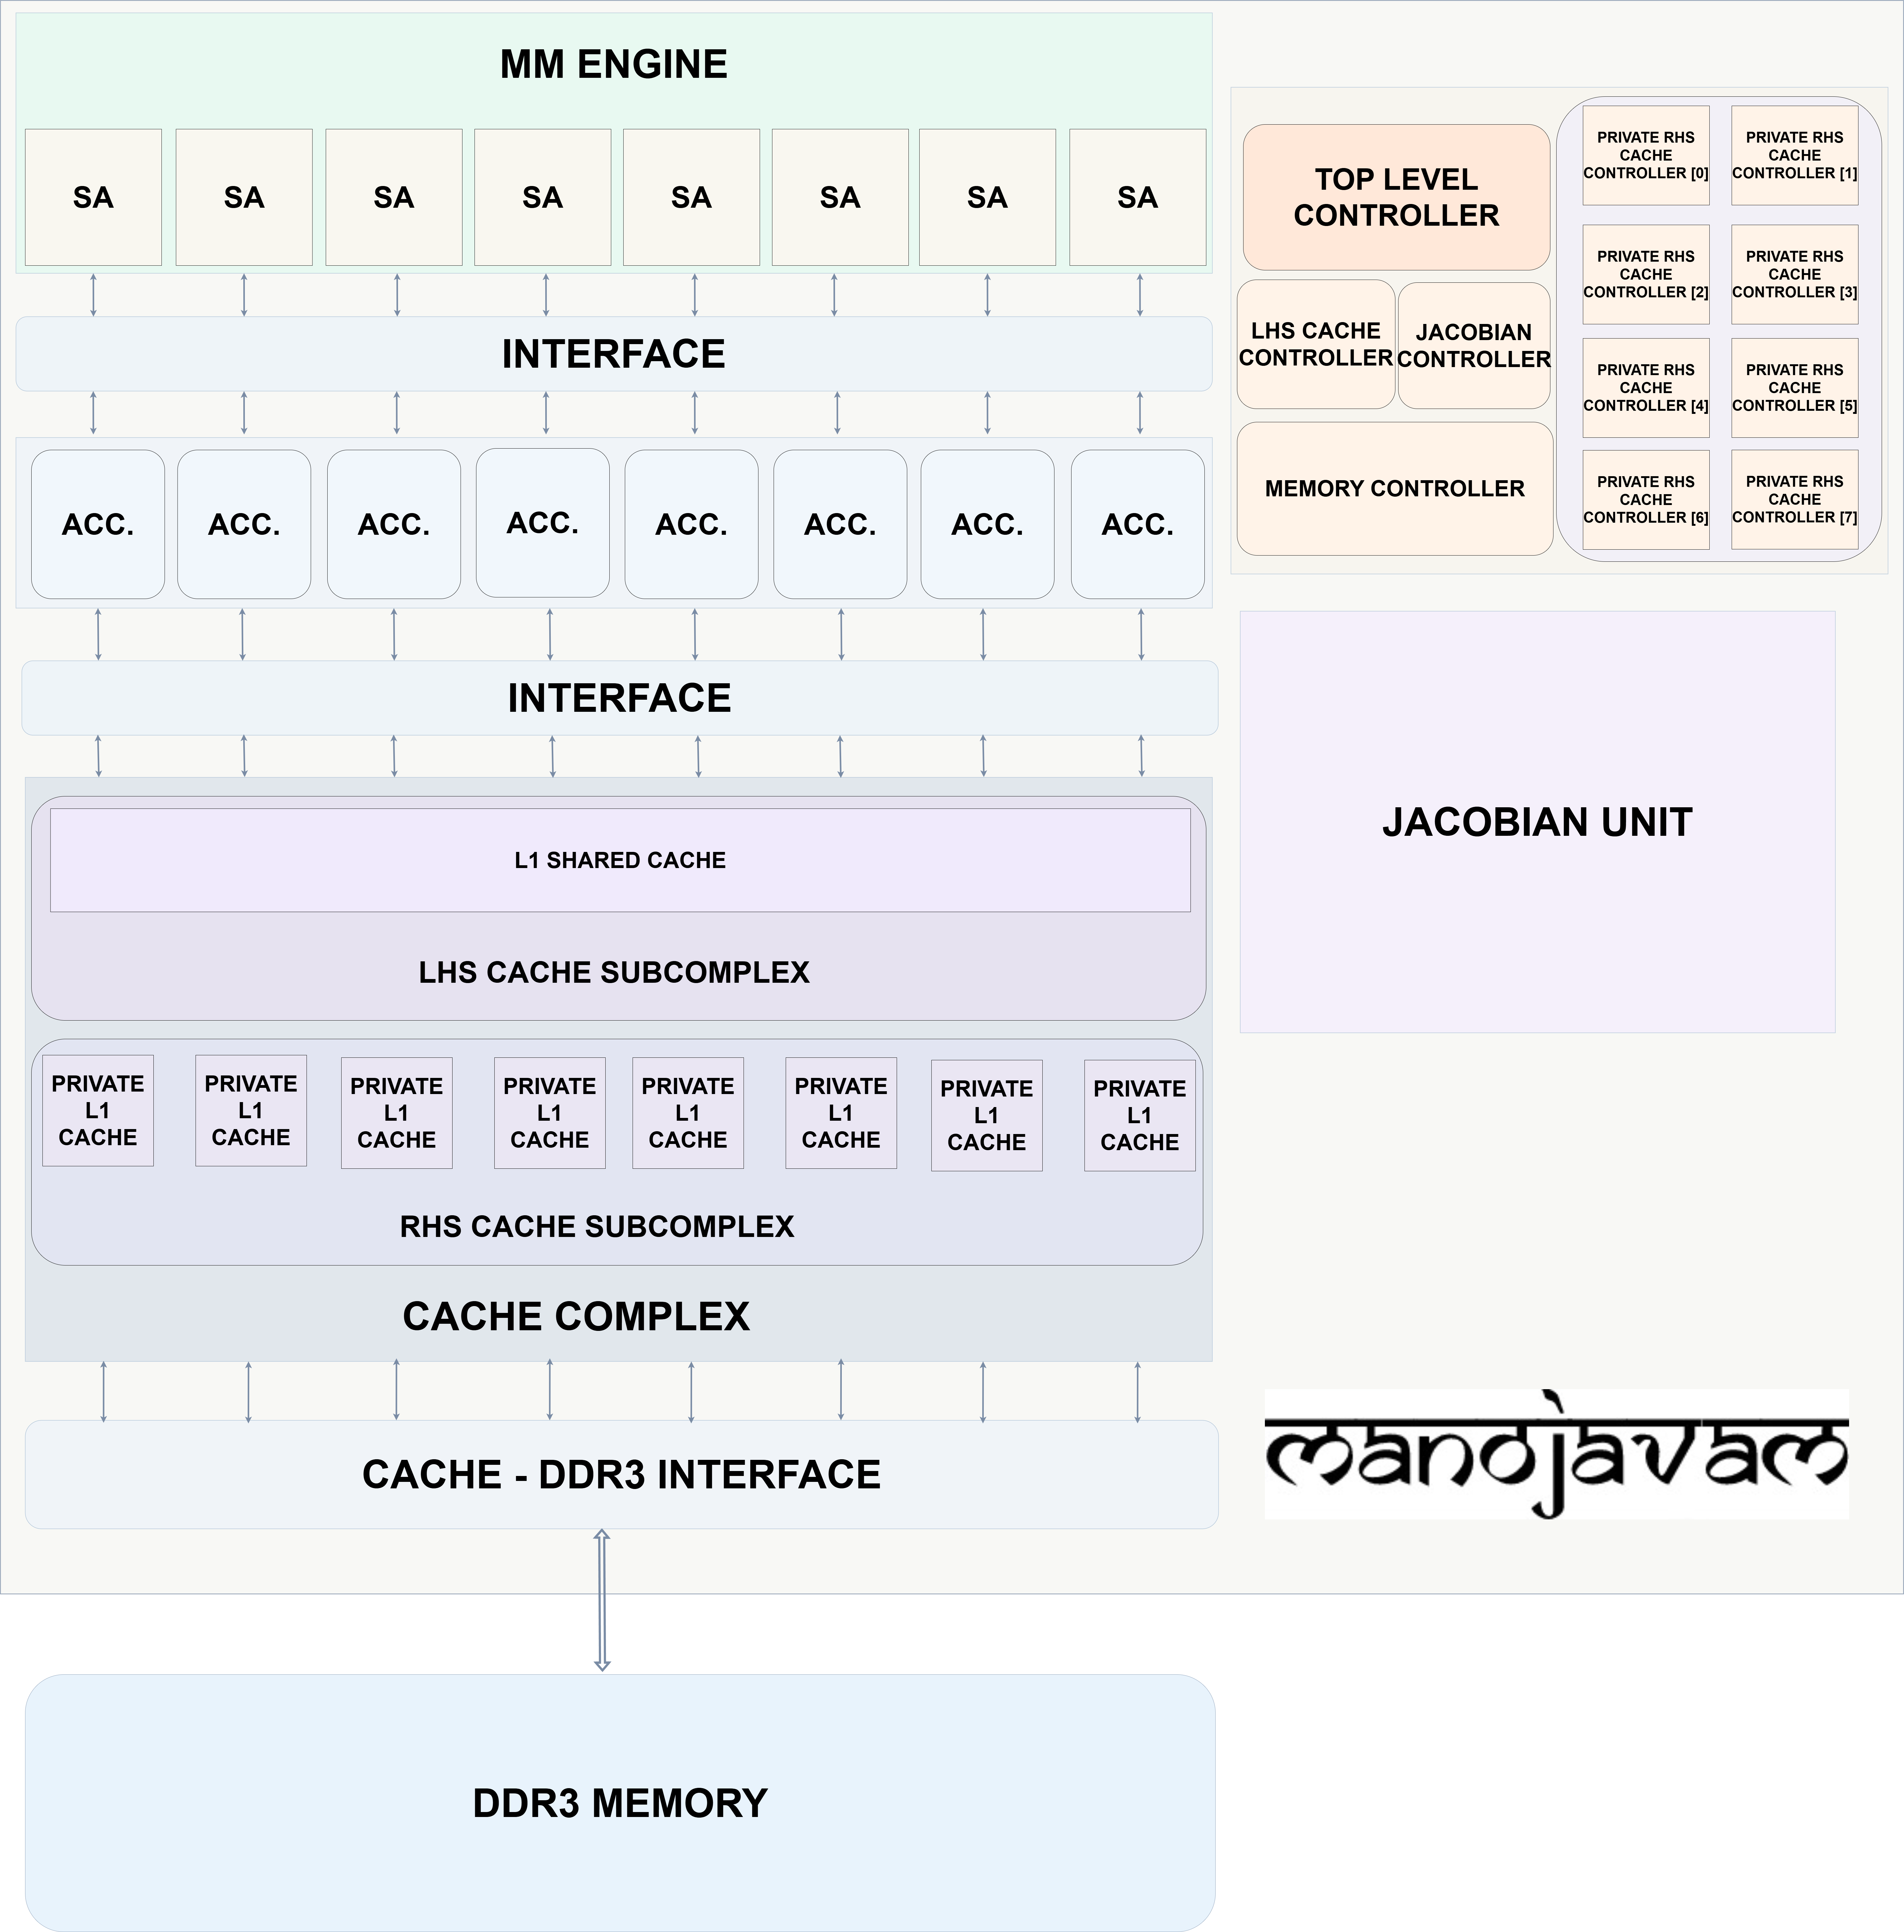
\includegraphics[scale = 0.05]{Figures/manojavam_architecture_v4.png}}
	\caption{High Level Architecture of Manojavam}
	\label{fig:manojavam high level architecture}
\end{figure}

\section{Matrix Multiplication Engine}
The Covariance Matrix Computation Unit is tasked with constructing the symmetric matrix $C = X^{T}X$ where $X$ is the input dataset matrix with mean-subtracted and standardized values. In PCA, this matrix encodes the pairwise correlations between input features and forms the foundation for identifying dominant eigenvectors. Due to the high dimensionality and streaming nature of ML datasets, direct computation of $X^{T}X$ is memory- and compute-intensive. Manojavam addresses this challenge using a tiled matrix multiplication approach, where the input matrix $X$ is divided into a series of smaller 4×4 operand tiles, allowing submatrix-level parallel processing and spatial data reuse.

These tiles are streamed into a Matrix Multiplication Engine (MM Engine) comprising eight independent 4×4 systolic arrays, each designed to operate in parallel on a different tile pair. Systolic arrays are chosen for their regular structure and pipelined data movement, which reduces control complexity and maximizes throughput. Each array follows a weight-stationary dataflow model, where one operand (typically $X^{T}$) is held stationary within the array registers, while the second operand (typically $X$) flows through the pipeline. This model enables each multiply-accumulate (MAC) unit to reuse its stored operand multiple times, significantly reducing memory bandwidth requirements and off-chip traffic\cite{chap3-2}.

Large-scale matrix multiplication poses a fundamental bottleneck in hardware accelerators due to limited on-chip memory and compute parallelism. Manojavam addresses this challenge through block streaming matrix multiplication, shown in Fig.\ref{fig:tiled-MM}. It is a technique that decomposes large input matrices into smaller, fixed-size tiles — typically matching the size of the systolic array (e.g., 4×4 blocks). These tiles are streamed sequentially through a systolic compute fabric, allowing partial products to be accumulated incrementally across time without requiring the full matrix to reside on-chip. This tiling approach drastically reduces memory bandwidth pressure and allows effective reuse of operands stored in local buffers\cite{chap3-1}. Moreover, by orchestrating tile loading and compute through a staged controller and cache hierarchy, Manojavam overlaps data transfer with computation, ensuring that the processing elements remain fully utilized. This technique enables the accelerator to scale to arbitrarily large matrices within the limited BRAM resources of the FPGA, thereby making high-dimensional covariance computations and PCA viable even under strict hardware constraints.

\begin{figure}
	\centerline{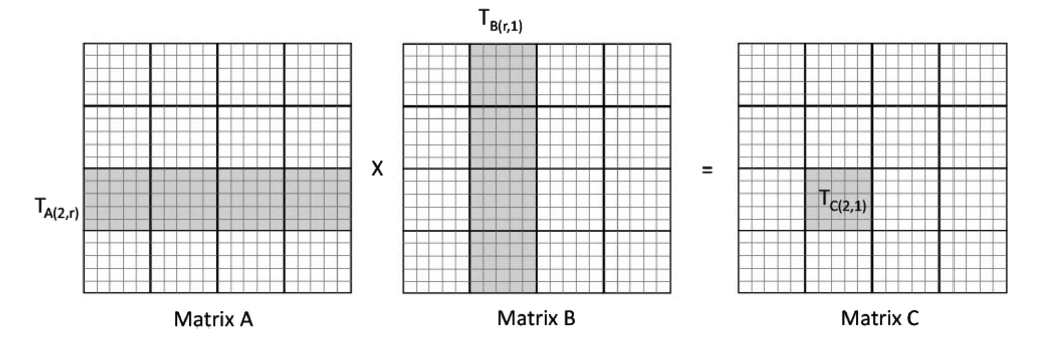
\includegraphics[scale = 0.75]{Figures/tiled_MM.png}}
	\caption{Illustration of Tiled Matrix Multiplication}
	\label{fig:tiled-MM}
\end{figure}

The systolic arrays process operand tile pairs in a wavefront pattern, where rows of $X^{T}$
and columns of $X$ are sequentially injected into the array, and intermediate products are propagated and summed through the grid of MAC units. The output of each array is a 4×4 partial product matrix corresponding to a block of the full covariance matrix. These partial products are not stored directly; instead, they are routed to a corresponding matrix accumulator, which collects and accumulates the results across multiple tile passes. Each accumulator is mapped one-to-one with a systolic array and implements a register or BRAM-based accumulation buffer, capable of holding intermediate values until all contributing tile products for that block have been processed.

Operand tiles are delivered to each systolic array through a structured input stream managed by Matrix Padding Units. These units take flattened 1D representations of the matrix stored in memory and reshape them into 2D tile structures, ensuring that operands are correctly aligned for the systolic pipeline. This is depicted in Fig.\ref{fig:systolic_array_setup}. Additionally, the padding units handle zero-padding for tiles at the matrix boundary when the input dimensions are not multiples of 4. This abstraction simplifies control logic and guarantees correctness across arbitrary input sizes.

\begin{figure}
	\centerline{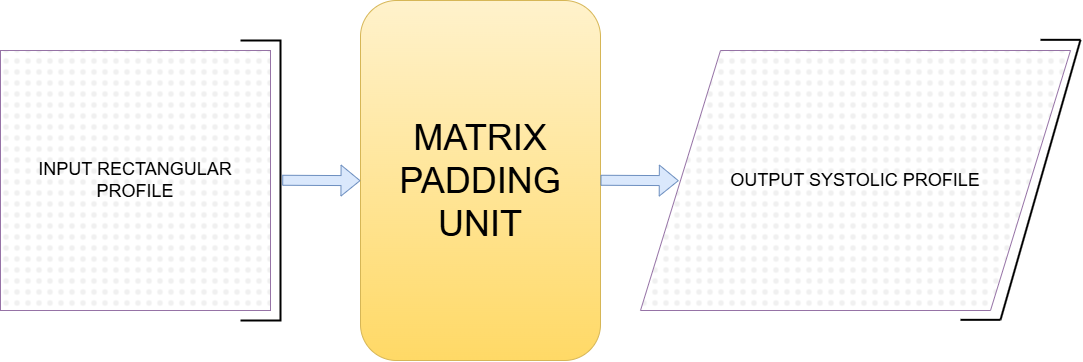
\includegraphics[scale = 0.35]{Figures/systolic_array_setup.png}}
	\caption{Systolic Operand Setup by Matrix Padding Units}
	\label{fig:systolic_array_setup}
\end{figure}

To further optimize resource usage, the systolic arrays are built using a hybrid MAC structure. Each 4×4 array contains both DSP-based MAC units, which offer high-speed multiplication, and LUT-based MAC units, which offer area efficiency and configurability. This hybrid approach provides flexibility for fine-grained performance tuning based on matrix size, input bit-widths, and target frequency constraints. For example, heavier matrix blocks can be assigned to DSP-enhanced arrays, while lighter or repetitive blocks can be processed using LUT-based arrays to conserve FPGA DSP slices.

The MM Engine is designed to be modular and scalable. Since the design partitions the full matrix computation into smaller tiles, larger matrices (e.g., 1024×1024 or 1000×4) can be processed iteratively by looping over tiles and summing partial results through the matrix accumulators. This design supports a streaming compute model, where the covariance matrix is constructed incrementally without the need to store the entire input matrix or intermediate products in memory. As a result, the engine is well-suited for machine learning workloads where datasets are large, memory access is costly, and hardware parallelism is critical for real-time performance.    

The Matrix Multiplication Engine (MM Engine) is not only central to covariance matrix computation but also serves a dual-purpose role in the broader architectural flow of Manojavam. A critical design feature of the accelerator is the datapath-level reuse of this MM Engine during the eigendecomposition phase of PCA, specifically for performing Givens rotations as part of the Jacobi method. Once the covariance matrix has been constructed, the rotation phase begins, requiring transformations of the form $C^{'} = R^{T}CR$ and $V=VR$, where $R$ is a Givens rotation matrix computed to zero out the selected off-diagonal element of the covariance matrix.

Rather than implementing a separate hardware unit for these matrix-matrix multiplications, the architecture repurposes the same systolic arrays used in the covariance computation phase. This reuse is made possible by the input tile streaming abstraction, where operand tiles—regardless of their mathematical meaning (dataset blocks, covariance matrix rows, or Givens rotation matrices)—can be streamed into the systolic arrays through the same input pipeline, formatted using the Matrix Padding Units. This modularity allows the MM Engine to operate seamlessly across different computation phases without any structural changes.

A single mode control signal, propagated from the top-level controller, dynamically configures the MM Engine to switch between covariance mode and rotation mode. In covariance mode, the engine performs $X^{T}X$ using input tiles of the dataset; in rotation mode, it processes either $R^{T}C$, $CR$ or $VR$ depending on the sweep step in the Jacobi iteration. The operand cache controllers and memory access paths are also adjusted according to the mode, ensuring that operand delivery, accumulation policies, and write-back paths remain consistent with the target operation.

This design approach—reusing the MM Engine across both the covariance computation and the Jacobi rotation stages—offers a practical solution to reducing hardware overhead and simplifying system integration. By utilizing the same systolic datapath for different phases of PCA, the design avoids redundant hardware instantiations, resulting in a more resource-conscious implementation. The ability to support both operations through common tile streaming and buffer management also helps in maintaining a uniform interface for operand delivery and accumulation. Mode-based reconfiguration of operand sources and control signals ensures functional flexibility without significantly increasing architectural complexity. Overall, the reuse of the MM Engine reflects a thoughtful design trade-off between generality and specialization, aligning with the broader goals of area efficiency and functional completeness in hardware accelerators intended for matrix-intensive workloads. 

\section{Jacobian Unit Architecture}
The Jacobian Unit in the Manojavam architecture, depicted in Fig.\ref{fig:jacobian unit architecture}, is responsible for orchestrating the core numerical operations in the Jacobi method for Singular Value Decomposition (SVD), which underpins the eigendecomposition phase of Principal Component Analysis (PCA). The unit enables iterative diagonalization of the symmetric covariance matrix by computing successive Givens rotations that eliminate off-diagonal terms. This hardware-accelerated unit is composed of three tightly coupled submodules — the Data Lookup Engine (DLE), CORDIC Kernels, and the Givens Engine — which together facilitate high-throughput, low-latency execution of the Jacobi algorithm without resorting to software-driven matrix traversal or off-chip computation.

\begin{figure}
	\centerline{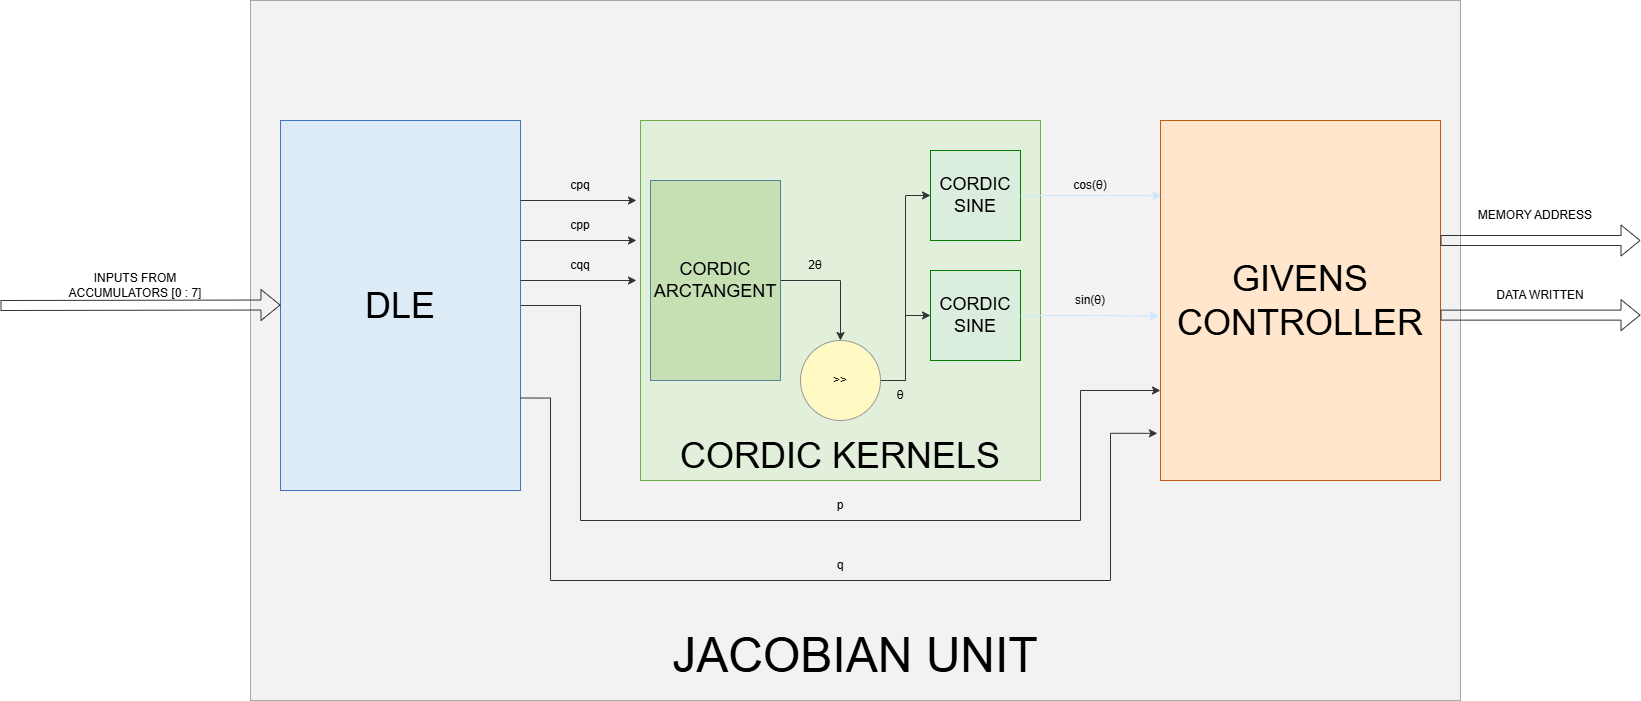
\includegraphics[scale = 0.3]{Figures/Jacobian Unit.png}}
	\caption{Jacobian Unit Architecture}
	\label{fig:jacobian unit architecture}
\end{figure}

\subsection{Data Lookup Engine (DLE)}
The Data Lookup Engine (DLE) is a unique architectural innovation in Manojavam, specifically designed to identify the largest off-diagonal entry in the symmetric covariance matrix $C$, which is the target of each Jacobi sweep. Unlike conventional designs that rely on off-chip memory or multiple on-chip reads to traverse the matrix and extract this value, the DLE operates in-line with the accumulation path of the matrix multiplication unit. As partial sums for each matrix tile are generated during block streaming multiplication, the DLE snoops into these intermediate values and selectively captures the relevant ones based on the row-block and column-block identifiers.

To ensure that only valid off-diagonal elements cpq are considered, the DLE incorporates logic to ignore diagonal entries ($c_{pp}$, $c_{qq}$) and focuses only on entries where $p \neq q$. For example, during the accumulation of row block $R_{0}$, only entries from accumulators corresponding to columns 1 through $N$ are considered, with accumulator 0 (holding $c_{pp}$) explicitly excluded. This dynamic filter is implemented using row-wise masking and loop counters governed by the Jacobian Controller.

The DLE maintains a running maximum register, which stores the current best candidate $c_{pq}$ and its associated diagonal elements $c_{pp}$, $c_{qq}$, as well as the corresponding indices $p$ and $q$. These values are updated if a newly received cpq is of greater absolute magnitude than the current maximum. Once a complete row sweep is done, the DLE asserts a ready flag and outputs the final triplet. This mechanism eliminates the need for matrix reads post-accumulation and tightly couples the matrix traversal logic with the systolic dataflow, making it highly efficient in both time and energy.

\subsection{CORDIC Kernels}
After the DLE has identified the indices $(p, q)$ and corresponding values $c_{pq}$, $c_{pp}$, and $c_{qq}$, the next stage involves computing the rotation angle $\theta$ required to construct the Givens rotation matrix $R$. This is done using the equation:

\begin{equation}
	\theta = \frac{1}{2}\arctan(\frac{2.c_{pq}}{c_{pp} - c_{qq}})
	\label{eq:rotation-angle-equation}
\end{equation}

This computation typically involves a floating-point division and arctangent operation, which are hardware-expensive. Instead, Manojavam employs CORDIC (Coordinate Rotation Digital Computer) kernels — a class of shift-and-add algorithms that efficiently compute trigonometric functions using only adders, shifters, and a lookup table.

The CORDIC engine is implemented as a 3-stage pipeline:
\begin{itemize}
	\item Stage 1 computes the arctangent of the normalized input.
	\item Stage 2 and 3 compute the sine and cosine of the resulting angle using vector rotation mode. 
\end{itemize}

These kernels work in fixed-point arithmetic, carefully scaled to match the datapath width of Manojavam while preserving numerical stability. Because of pipelining, a new angle can be fed into the CORDIC engine every few clock cycles, and once the latency is absorbed, the unit can achieve near-one-angle-per-cycle throughput. This design is ideal for iterative eigendecomposition, where hundreds of such angles may be computed across multiple Jacobi sweeps.

The $sin(\theta)$ and $cos(\theta)$ values are then forwarded to the Givens Engine, which uses them to construct the sparse rotation matrix.

\subsection{Givens Engine}
The Givens Engine is responsible for generating and storing the actual Givens rotation matrix $R$ using the rotation angle $\theta$. In the Jacobi method, the Givens matrix is an identity matrix with four modified elements at $[p][p]$, $[q][q]$, $[p][q]$, and $[q][p]$, which are set to:
\begin{enumerate}
	\item $R_{pp} = R_{qq} = cos(\theta)$
	\item $R_{pq} = sin(\theta)$
	\item $R_{qp} = -sin(\theta)$
\end{enumerate}

This localized modification is sufficient to apply a plane rotation in the $(p,q)$ subspace of the matrix, progressively zeroing out the off-diagonal term $c_{pq}$. The Givens Engine stores this matrix in a dual-port RAM, enabling simultaneous read and write operations during iterative construction and rotation phases. This storage structure is accessed by downstream matrix multiplication units for computing:
\begin{equation}
	C^{'} = R^{T}CR
\end{equation}

\begin{equation}
	V = VR
\end{equation}

The Givens Controller synchronizes matrix updates and triggers operand movement within the memory hierarchy. It generates select signals to update only relevant portions of the Givens matrix, thereby avoiding unnecessary re-initialization. Once the matrix is ready, a mode signal is broadcast to all computational units, switching the pipeline from covariance accumulation to rotation mode.

To minimize performance overhead, the engine also preloads the next Givens rotation during the computation of the current matrix transformation, enabling overlap of angle generation and matrix rotation — a technique analogous to prefetching in cache systems.

\section{Cache Subsystem}
Efficient memory access plays a critical role in sustaining the performance of high-throughput accelerators. In Manojavam, where multiple 4×4 systolic arrays operate in parallel, the design of the memory subsystem is crucial for maintaining computational flow without stalling. To support continuous and parallel tile streaming across compute stages, Manojavam implements a dual-tier cache hierarchy—consisting of L1 and L2 caches—architected specifically to match the operand reuse patterns that arise in block-wise matrix multiplication.

The left-hand side (LHS) operands, such as the rows of $X^{T}$ during covariance matrix computation or $R^{T}$ during rotations, are typically reused across multiple columns or matrix blocks. This temporal locality makes them good candidates for shared caching. Accordingly, all LHS operands are stored in a shared L1 cache, which is accessible to all eight systolic arrays through a broadcast-style access network. This shared architecture reduces memory footprint, eliminates unnecessary duplication of frequently used data, and simplifies coherency management for read-only accesses. The shared cache also includes address decoding and basic arbitration logic to allow synchronized reads from multiple consumers.

In contrast, the right-hand side (RHS) operands—including the columns of $X$, the evolving covariance matrix $C$, or the rotation matrix $R$—are typically unique to each systolic array during a particular compute cycle. These operands do not exhibit the same reuse pattern and are thus stored in private L1 caches, with each cache directly connected to one of the eight systolic arrays. This private caching scheme eliminates the need for read arbitration, enables concurrent data delivery, and supports tile-specific prefetching. Each private cache is configured to hold an entire 4×4 operand tile in a row-aligned format, enabling burst-mode reads to feed systolic inputs efficiently.

To optimize data delivery, the cache stores each operand tile in a row-major layout rather than as a raw matrix. This means each row of the 4×4 tile is stored contiguously, allowing the systolic array to receive an entire row of inputs in a single read cycle instead of multiple sequential accesses. By reducing the number of memory fetches from four to one per row, this approach significantly improves data throughput, reduces latency, and better aligns with the streaming nature of the systolic array’s pipeline.

All L1 caches—both shared and private—are backed by a common L2 memory pool, implemented as a dual-ported block RAM module or connected externally via a DDR3 memory interface. This L2 layer serves as the staging area for incoming operand tiles and also receives the accumulated results post-computation. A dedicated memory controller coordinates requests from the cache complex and enforces proper sequencing for tile fetch and write-back operations. To reduce memory bandwidth pressure and prevent redundant data movement, Manojavam employs selective cache write policies tailored to the two major computation phases.

During covariance matrix computation, a write-around policy is used for the RHS caches. In this policy, new tiles are written directly to memory without allocating space in the cache unless the data is expected to be reused. This minimizes cache pollution and allows each private cache to retain active working tiles without being overwritten by one-time-use data.

In the rotation phase, a write-validate policy is enforced, especially for matrix $C$ and the evolving eigenvector matrix $V$. This policy ensures that when matrix updates are written to memory, the corresponding cache entries are marked valid, but no fetch-on-write is triggered. This reduces unnecessary memory traffic while still maintaining coherency. The system relies on the fact that the MM Engine overwrites the same tile locations in a predictable schedule, making manual validation sufficient for correctness.

Tile streaming in this memory hierarchy is managed via a controller-driven tile scheduler, which issues operand fetch signals to the caches in a fixed loop structure. This streaming-friendly model avoids complex memory dependency tracking and supports pipeline-friendly operand delivery to the systolic arrays. Furthermore, by isolating frequently reused operands from ephemeral ones, the design achieves a balance between temporal locality exploitation and parallel access concurrency, both of which are critical in matrix-intensive computation.

The overall memory system is designed to scale with matrix size, supporting tile dimensions beyond the capacity of L1 caches by fetching on demand and buffering partial results for accumulation. It minimizes idle cycles in the datapath, maintains high utilization of the systolic arrays, and simplifies the scheduling logic by clearly separating cache responsibilities according to operand behavior. This architecture, while lightweight in its logic and buffering requirements, forms a central enabler of Manojavam’s streaming and reuse-aware compute strategy.   

\section{Controller Design and Hierarchy}
The efficient operation of the Manojavam PCA accelerator heavily relies on a well-structured controller hierarchy that orchestrates data flow, synchronization, and computation across multiple compute units and memory subsystems. The hierarchy is designed to modularize control responsibilities, simplify synchronization, and enable scalable management of parallel processing elements. The controller hierarchy consists of four primary levels:

\subsection{Top-Level Controller}
At the apex of the control architecture lies the Top-Level Controller, which functions as the master coordinator for the entire design. Its primary responsibility is to synchronize all subordinate controllers, ensuring smooth handshaking and timing alignment between the different units—namely, the shared LHS cache controller, the private RHS cache controller complex, and the Jacobian Unit controller. The top-level controller orchestrates the overall flow of computation phases, triggers operand fetch and store operations, and manages global start, stop, and reset signals. By maintaining a centralized state machine, this controller ensures that the system operates in a lockstep manner, preventing data hazards and ensuring consistent data availability across all compute pipelines.

\subsection{LHS Shared Cache Controller}
The LHS Shared Cache Controller is responsible for managing all operations related to the left-hand side (LHS) shared cache. This includes handling broadcast reads to multiple systolic arrays, address decoding, cache coherence management for read-only data, and arbitration for simultaneous access requests. Given that the LHS operands exhibit high temporal reuse and are shared across all eight systolic arrays, this controller plays a critical role in reducing redundant memory traffic and maintaining consistent operand delivery. It schedules tile fetches from the L2 memory into the shared cache and coordinates cache line validation to ensure the freshest data is available to the compute units.

\subsection{Private RHS Cache Controller Complex}
The Private RHS Cache Controller Complex comprises eight independent private cache controllers, each dedicated to managing one of the eight private RHS caches linked to the individual systolic arrays. Each private cache controller handles local operand prefetching, cache line allocation, and write-back policies tailored to the right-hand side (RHS) operands that are unique per systolic array during computation. This modular organization enables concurrent and conflict-free memory accesses, as each controller operates autonomously with minimal synchronization overhead. The complex also enforces the selective write-around and write-validate policies, optimizing cache utilization based on operand reuse characteristics in covariance and rotation phases.

\subsection{Jacobian Controller}
The Jacobian Controller oversees the operation of the Jacobian Unit, which is responsible for implementing the Jacobi eigendecomposition algorithm during the PCA process. This controller manages iterative sweep operations, controls rotation matrix generation via CORDIC engines, and coordinates data movement between the rotation unit and the matrix multiplication engine. It synchronizes the execution of Givens rotations and ensures correct sequencing of eigenvector updates. By tightly integrating with the top-level controller, the Jacobian Controller maintains coherent operation between the covariance computation phase and the rotation phase, enabling smooth pipeline transitions.

\begin{comment}
\section{Contents of this Chapter}
This chapter should contain the following sections and subsections in detail.
\begin{enumerate}
\item Specifications for the Design
\item Pre analysis work for the design or Models used
\item Design methodology in detail
\item Design Equations
\item Experimental techniques (if any)
\end{enumerate}
Apart from the aforementioned sections, you can add sections as per the requirements of the project in consultation with your guide.
\end{comment}

Chapter 3 presents the comprehensive design methodology and specifications that underpin both the FPGA Architectural Exploration and the development of the Manojavam PCA accelerator. It begins by detailing the specific design requirements and objectives for evaluating diverse FPGA architectures using the VTR toolchain, followed by the modeling approaches employed to accurately represent targeted FPGA configurations. The chapter outlines the systematic methodology adopted to perform architectural exploration, including synthesis, placement, and routing workflows, alongside the critical performance and area analysis metrics supported by relevant equations. The focus then shifts to the architectural design of the Manojavam accelerator, describing its core components in detail — the matrix multiplication engine, which leverages multiple 4×4 systolic arrays for high-throughput matrix operations; the Jacobian unit, responsible for eigendecomposition via Jacobi rotations; and the cache subsystem, architected to optimize operand reuse and data streaming. Finally, the controller hierarchy is elaborated, highlighting the modular control scheme that ensures synchronized operation and efficient data flow across the compute and memory units. Together, these sections form the foundation for both the FPGA exploration and accelerator implementation, linking theoretical design choices with practical hardware realization.

\begin{comment}
\section{Paraphrasing}
When you paraphrase a written passage, you rewrite it to state the essential ideas in your own words. Because you do not quote your source word for word when paraphrasing, it is unnecessary to enclose the paraphrased material in quotation marks. However, the paraphrased material must be properly referenced because the ideas are taken from someone else whether or not the words are identical. 

Ordinarily, the majority of the notes you take during the research phase of writing your report will paraphrase the original material. Paraphrase only the essential ideas. Strive to put original ideas into your own words without distorting them."

\section{Quotations}
When you have borrowed words, facts, or idea of any kind from someone else's work, acknowledge your debt by giving your source credit in footnote (or in running text as cited reference). Otherwise, you will be guilty of plagiarism. Also, be sure you have represented the original material honestly and accurately. Direct word to word quotations are enclosed in quotation marks."

\vspace{0.75cm}

 \textbf{The chapters should not end with figures, instead bring the paragraph explaining about the figure at the end followed by a summary paragraph.}
\end{comment}

\begin{comment}
After elaborating the various sections of the chapter (From Chapter 2 onwards), a summary paragraph should be written discussing the highlights of that particular chapter. This summary paragraph should not be numbered separately. This paragraph should connect the present chapter to the next chapter.  
\end{comment}